\documentclass{article}
\usepackage{babel}
\usepackage{amssymb,amsmath}
\usepackage{graphicx}
\usepackage[utf8]{inputenc}	

\begin{document}



\section{Ejercicio 7}

\subsection{Introducci\'on}
\noindent
En la presente sección se desarrolla la implementaci\'on de dos contadores de 3 bits, uno sincr\'onico y uno asincr\'onico. Se analizan diferencias de funcionamiento entre ambos y se cuantifican par\'ametros importantes en cuanto a la operaci\'on de cada uno.

%\todo{alargar intro y ver si se cuantifican parametros varios o solo la maxima velocidad de operacion}

\subsection{Diseño}
\noindent
A continuaci\'on se muestra

\subsubsection{Contador asincr\'onico}
\label{ej7_sec:cont_asinc}
\noindent
Para la implementaci\'on del contador asincr\'onico se parte del circuito de la Figura 	\ref{ej7_fig:asinc_init}. Tomando N = $Q_2 Q_1 Q_0$, este contador cuenta de 0 a 7 y luego vuelve a comenzar. Se trata de un contador asincr\'onico porque, como se puede observar, s\'olo el primer Flip-Flop tiene su entrada de CLK conectada a la señal de clock, mientras que los dem\'as se activan con un flanco ascendente de $\overline{Q_{n-1}}$, es decir, un flanco descendente de $Q_{n-1}$. Por lo tanto, en el caso de que tenga que activarse el \'ultimo Flip-Flop, a \'este le llega el flanco ascendente luego del retardo de los dos primeros, con lo que no hay sincronismo. \\
%
\begin{figure}[H]
%\begin{figure}[hb!]
	\centering
	\resizebox{0.7\linewidth}{!}{
			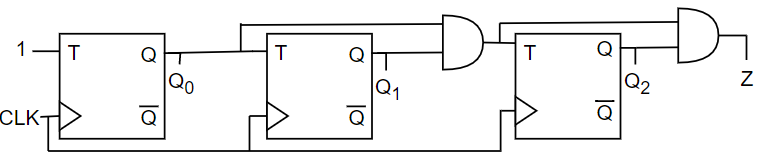
\includegraphics{figs/Ej7/ej7_sinc_circ.PNG}	
	}
	\caption{Circuito de un contador asincr\'onico de 3 bits.}
	\label{ej7_fig:asinc_init}
\end{figure}
%
Como se dispone de circuitos integrados Flip-Flop D, se utilizan \'estos para obtener los Flip-Flop T que utiliza el circuito. Para ello, se busca una funci\'on l\'ogica que relacione la entrada T y la salida Q con la entrada D que debe tener el integrado para que el circuito se comporte como un Flip-Flop T. La tabla de verdad de dicha funci\'on se muestra en la Tabla \ref{ej7_tab:FFDaFFT}.
%
\begin{table}[H]
%\begin{table}[ht!]
\centering
\begin{tabular}{|c|c|c|}
\hline
\textbf{T} & \textbf{Q} & \textbf{D} \\ \hline
0          & 0          & 0          \\ \hline
0          & 1          & 1          \\ \hline
1          & 0          & 1          \\ \hline
1          & 1          & 0          \\ \hline
\end{tabular}
\caption{Tabla de verdad para hacer un FFT a partir de un FFD.}
\label{ej7_tab:FFDaFFT}
\end{table}
%
De la tabla de verdad se obtiene que:
%
\begin{equation}
	D = T \oplus Q
\end{equation}
%
Por lo tanto, se obtiene un Flip-Flop T mediante el circuito de la Figura \ref{ej7_fig:FFDaFFT}.
%
\begin{figure}[H]
%\begin{figure}[hb!]
	\centering
	\resizebox{0.7\linewidth}{!}{
		\includegraphics{ej7_ffd_fft.PNG}
%		\includegraphics{figs/Ej7/ej7_ffd_fft.PNG}
	}
	\caption{Circuito para hacer un FFT a partir de un FFD.}
	\label{ej7_fig:FFDaFFT}
\end{figure}
%
Utilizando 

\subsubsection{Contador sincr\'onico}
\noindent

...Al igual que en la Subsecci\'on \ref{ej7_sec:cont_asinc}, utilizando Flip-Flops D para realizar las Flip-Flops T, el circuito pasa a ser el de la Figura \ref{ej7_fig:asinc_circ_final}}

%
\begin{figure}[H]
%\begin{figure}[hb!]
	\centering
	\resizebox{0.7\linewidth}{!}{
		\includegraphics{}
	}
	\caption{Circuito del contador asincr\'onico con FFD.}
	\label{ej7_fig:asinc_circ_final}
\end{figure}
%

\subsection{Elecci\'on del IC}
\noindent
A la hora de la elecci\'on del circuito integrado (IC) a utilizar, se contaba con 

%
% CD4013: Dual D Type Flip Flop, CMOS,  RD [asynchronous reset-direct input]: active LOW
% 7474: Dual D positive edge triggered flip-flop,asynchronous preset and clear,  CD [asynchronous clear-direct input]: active HIGH
% hay 74LS74 (TTL) y 74HC74 (CMOS)

\subsection{An\'alisis de resultados}
\noindent

\subsection{Conclusi\'on}
\noindent

\end{document}